\documentclass{beamer}
\usepackage{listings}\usepackage[utf8]{inputenc}
\usepackage[T1]{fontenc}
\usepackage[french]{babel}
\usepackage{lmodern}
\usepackage{amsmath}
\usepackage{amssymb}
\usepackage{algorithm}
\usepackage{algpseudocode}
\usepackage{array}
\usepackage{pgf,tikz}
\usepackage{listings}
\usetikzlibrary{arrows}


\usetheme{Warsaw}
\title{Compression fractale}
\author{Pierre \textsc{Vigier} -- Frédéric \textsc{Wantiez}}
\institute{CentraleSupélec}
\date{29 mai 2017}

\expandafter\def\expandafter\insertshorttitle\expandafter{%
  \insertshorttitle\hfill%
  \insertframenumber\,/\,\inserttotalframenumber}
  
\AtBeginSection[]{
  \begin{frame}
  \vfill
  \centering
  \begin{beamercolorbox}[sep=8pt,center,shadow=true,rounded=true]{title}
    \usebeamerfont{title}\insertsectionhead\par%
  \end{beamercolorbox}
  \vfill
  \end{frame}
}

\AtBeginSubsection[]{
  \begin{frame}
  \vfill
  \centering
    \usebeamerfont{title}\insertsubsectionhead\par%
  \vfill
  \end{frame}
}

\begin{document}

\begin{frame}
\titlepage
\end{frame}

\begin{frame}{Théorèmes fondamentaux}
\begin{block}{Théorème du point fixe pour une application contractante}
Soit $(E, d)$ un espace métrique complet et $f : E \rightarrow E$ une application $s$-contractante. $f$ a un unique point fixe $x_0$ et
$$\forall x \in E, \forall n \in \mathbb{N}, d(x_0, f^n(x)) \leq s^n d(x_0, x)$$
\end{block}

\begin{block}{Théorème du collage}
Soit $(E, d)$ un espace métrique complet et $f : E \rightarrow E$ une application $s$-contractante. Notons, $x_0$ le point fixe de $f$, on a alors :
$$\forall x \in E, d(x, x_0) \leq \frac{d(x, f(x))}{1-s}$$
\end{block}
\end{frame}

\begin{frame}{PIFS}
Soit $F = (L^2([0, 1]^2, \mathbb{R}), d_2)$ avec
$$\forall f, g \in F, d_2(f, g) = \int_{(x,y) \in [0, 1]^2}{|f(x, y) - g(x, y)|^2dxdy}$$
F est un espace métrique complet.
\begin{block}{Partitioned iterated function systems}
Pour $i \in \{1, ..., n\}$, soit $\tilde{w}_i : D_i \rightarrow R_i$ une translation affine où $D_i, R_i \subset [0, 1]^2$ sont des compacts. On pose pour $i \in \{1, ..., n\}$ :
$$w_i(f)(x, y) = s_i f(\tilde{w}^{-1}_i(x, y)) + o_i$$
Finalement, on pose $W : F \rightarrow F$ telle que :
$$\forall f \in F, W(f)(x, y) = w_i(x, y) \text{ si } (x, y) \in R_i$$
\end{block}
\end{frame}

\begin{frame}{Compression}
\begin{block}{Algorithme de compression}
\begin{itemize}
\item Segmenter $[0, 1]^2$ en $R_1, ..., R_n$ disjoints.
\item Segmenter $[0, 1]^2$ en $D_1, ..., D_N$.
\item Pour tout $R_i$, choisir un $D_{i_0}$ parmi les $D_1, ..., D_N$, une translation, $s_i$ et $o_i$ afin de minimiser $d_2(R_i, w_i(f)(D_{i_0}))$.
\item Retourner $w_1, ..., w_n$.
\end{itemize}
\end{block} 
\begin{center}
\begin{figure}
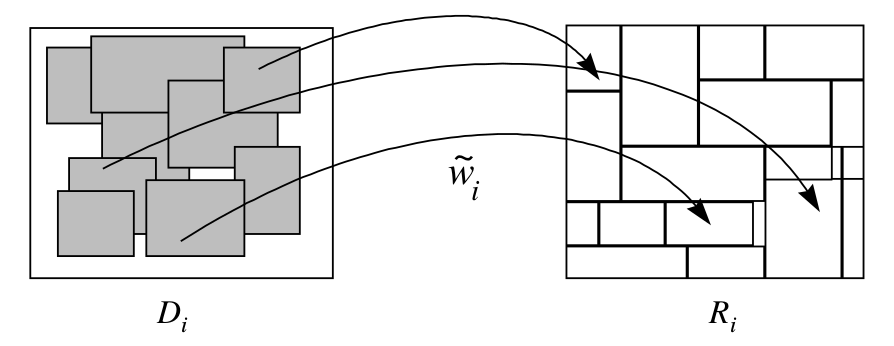
\includegraphics[scale=0.3]{images/pifs.png}
\end{figure}
\end{center}
\end{frame}

\begin{frame}{Décompression}
\begin{block}{Condition pour être une contraction}
Soit $\tilde{w} : (x, y) \mapsto Ax + b$ et $w : f \mapsto ((x, y) \mapsto s f(\tilde{w}^{-1}(x, y)) + o)$. $w$ est une contraction si $s \sqrt{|\det{A}|} < 1$.
Si tous les $(w_i)_i$ sont des contractions alors $W$ est une contraction. 
\end{block}

D'après les théorèmes du point fixe et du collage, le point fixe de $W$ va être une image proche de l'image d'origine.

\begin{block}{Décompression}
\begin{itemize}
\item Prendre une image quelconque $f$.
\item Calculer puis retourner $W^n(f)$.
\end{itemize}
\end{block}
\end{frame}

\begin{frame}{Exemple 1 : image en niveau de gris}
\begin{center}
\begin{figure}
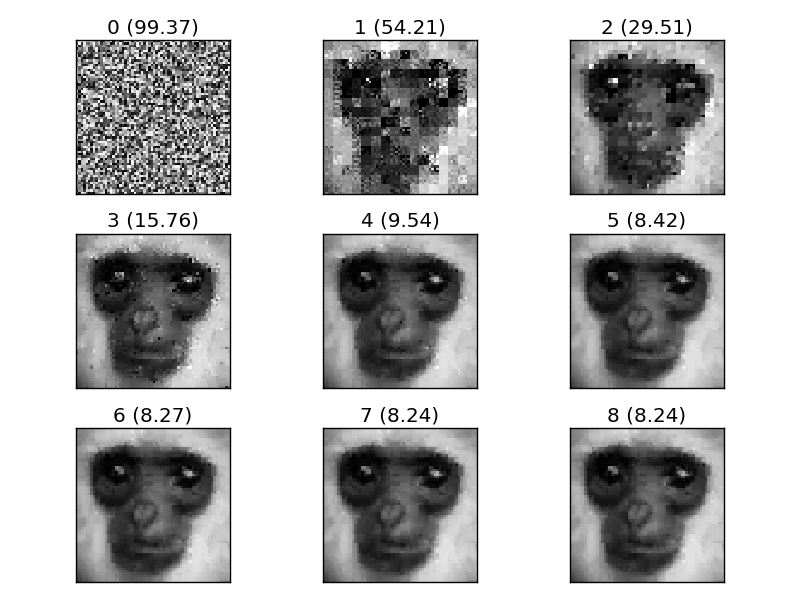
\includegraphics[scale=0.5]{images/monkey.png}
\end{figure}
\end{center}
\end{frame}

\begin{frame}{Exemple 2 : image en couleur}
\begin{center}
\begin{figure}
\begin{tiny}
\begin{tabular}{cc}
R & G \\
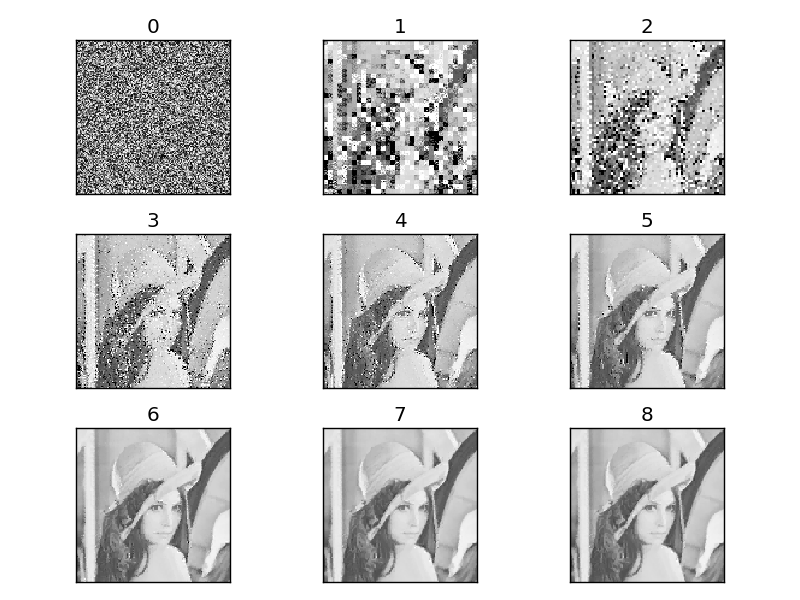
\includegraphics[scale=0.23]{images/lena_128_4_8/lena_r.png} & 
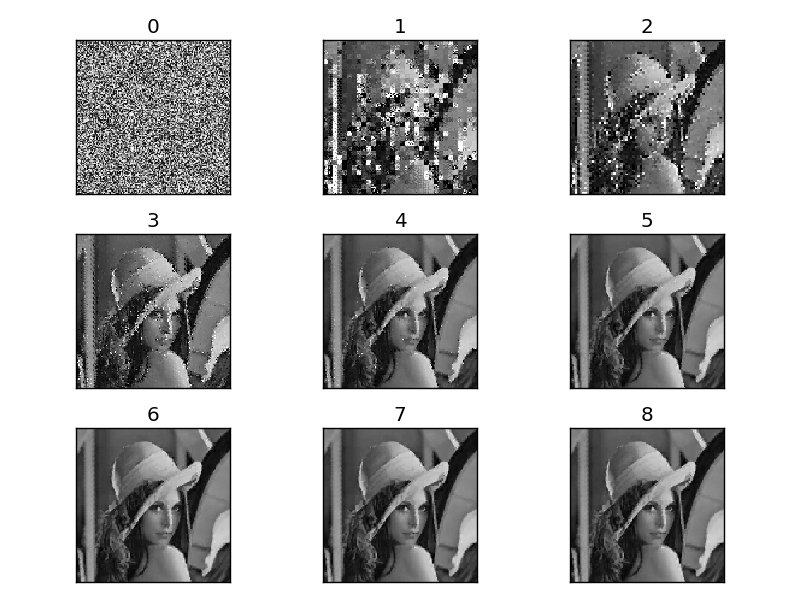
\includegraphics[scale=0.23]{images/lena_128_4_8/lena_g.png} \\
B & Total \\
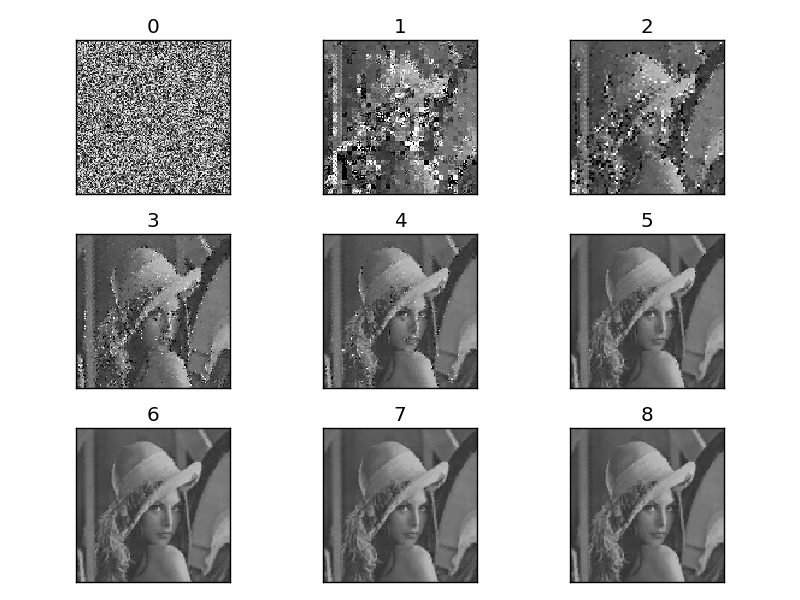
\includegraphics[scale=0.23]{images/lena_128_4_8/lena_b.png} & 
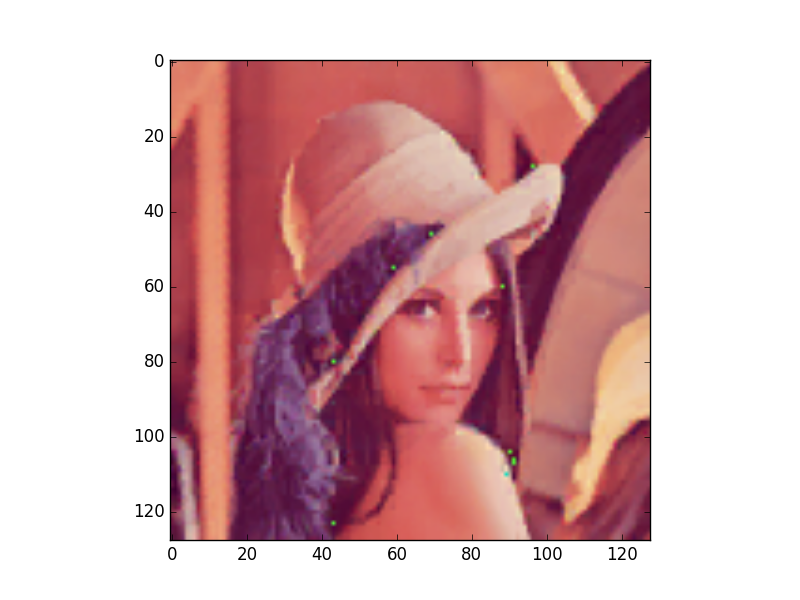
\includegraphics[scale=0.23]{images/lena_128_4_8/lena_128_4_8.png} \\
\end{tabular}
\end{tiny}
\end{figure}
\end{center}
\end{frame}

\begin{frame}{Performances}
	\begin{definition}{\textbf{Peak Signal to Noise Ratio (PSNR):}}
	Mesure de distorsion d'image, c'est une mesure locale i.e pixel par pixel:
	$$\text{PSNR} = 10\text{log}_{10}(\frac{d^2}{EQM})$$
	avec EQM l'erreur quadratique moyenne.
	\end{definition}
	\begin{definition}{\textbf{Structural Similarity (SSIM):}}
	Mesure de la dégradation structurelle de l'image après compression.
	Pour deux images $x$ et $y$:
	$$\text{SSIM}(x, y) = \frac{(2\mu_x\mu_y + c_1)(2\sigma_{xy} + c_2)}{(\mu_{x}^2 + \mu_{y}^2 + c_1)(\sigma_{x}^2 + \sigma_{y}^2 + c_2)} $$
	\end{definition}

\end{frame}

\begin{frame}{PSNR}
	\begin{center}
	\begin{figure}
	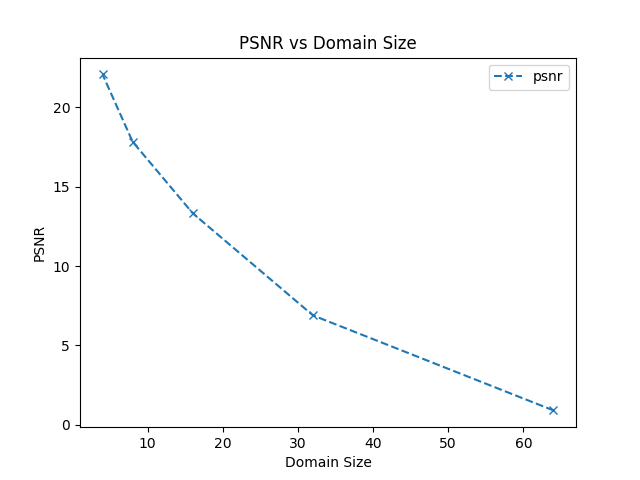
\includegraphics[scale=0.5]{images/error_rate_2.png}
	\caption{Distorsion en fonction de la taille des régions domaines $D_i$}
	\end{figure}
	\end{center}
\end{frame}

\begin{frame}{SSIM}
	\begin{center}
	\begin{figure}
	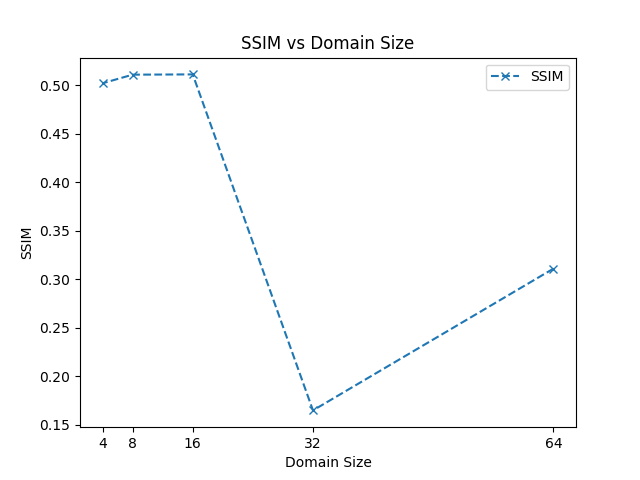
\includegraphics[scale=0.5]{images/error_SSIM.png}
	\caption{Erreur structurelle en fonction de la taille des régions domaines $D_i$}
	\end{figure}
	\end{center}
\end{frame}

\begin{frame}{Exemple : Image en niveau de gris}
\begin{center}
\begin{figure}
\begin{tiny}
\begin{tabular}{cc}
64 &  32\\
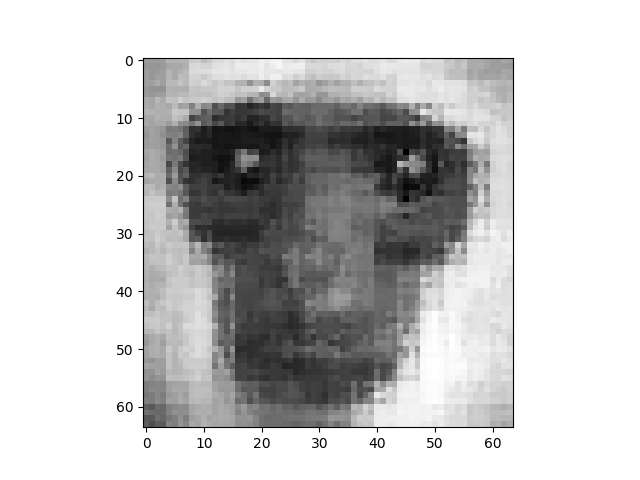
\includegraphics[scale=0.23]{images/monkey64-4.png} & 
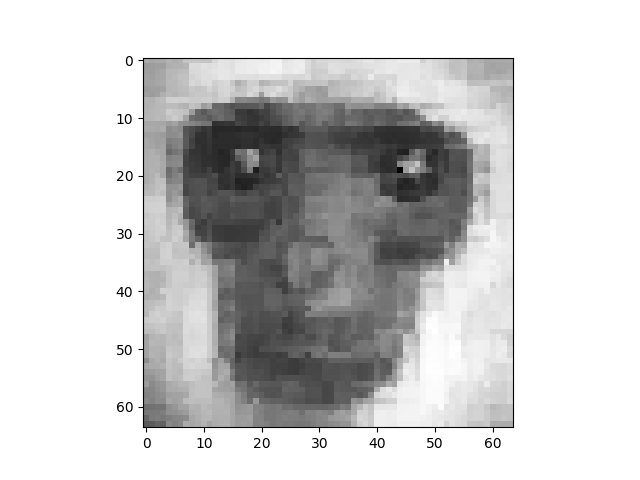
\includegraphics[scale=0.23]{images/monkey32-4.png} \\
16 & 8 \\
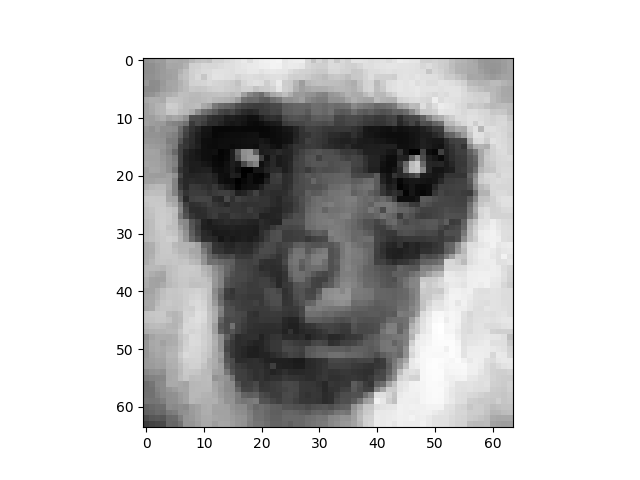
\includegraphics[scale=0.23]{images/monkey16-4.png} & 
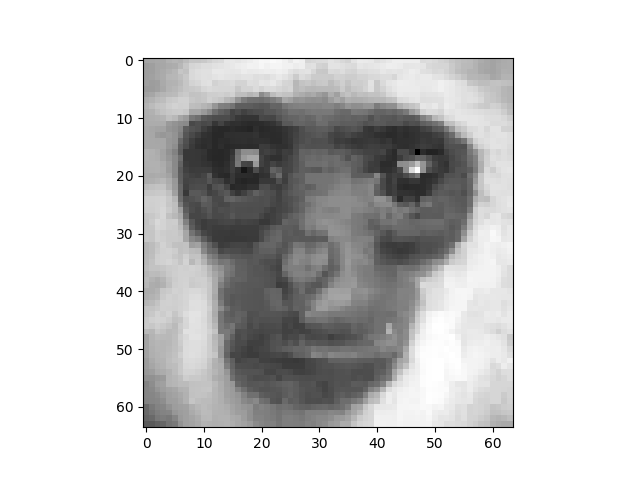
\includegraphics[scale=0.23]{images/monkey8-4.png} \\
\end{tabular}
\end{tiny}
\end{figure}
\end{center}
\end{frame}

\begin{frame}{Références bibliographique}
\begin{enumerate}
\item \textit{Compression Fractale d'Images} - Yuval Fischer, adaptation française de Matthieu Latapy
\item \textit{Fractal and Wavelet Image Compression Technique} - Stephen T. Welstead
\item \textit{Solution of an inverse problem for fractals and other sets} - M. F. Barnsley, V. Ervin, D. Hardin, J. Lancaster
\end{enumerate}
\end{frame}
\end{document}
